\section{Individual Contribution}
You should list the contribution and statements in the table \ref{individual contribution}.

\begin{table}[!h]
\centering
\caption{Individual Contribution}
\label{individual contribution}
    \begin{tabular}{ccc}
    \toprule
    \textbf{Name} & \textbf{UID} & \textbf{Contribution Statement} \\
    \midrule
    A & a & a\%, a's role and contributions here. \\
    B & b & b\%, b's role and contributions here. \\
    C & c & c\%, c's role and contributions here. \\
    D & d & d\%, d's role and contributions here. \\
    \bottomrule
    \end{tabular}
\end{table}

\section{Overall Result}
\subsection{Evaluation Result}
You should enter your results of the \textbf{evaluation dataset} of both tasks in the table \ref{eval}, e.g., accuracy for motion detection, and median MAE for breathing rate estimation.

\begin{table}[!h]
\centering
\caption{Overall Evaluation Result.}
\label{eval}
    \begin{tabular}{cc}
    \toprule
    \textbf{Evaluation Dataset} & \textbf{Result} \\
    \midrule
    Motion Detection & Your Accuracy (\%) \\
    Breathing Rate Estimation & Your median MAE (BPM) \\
    \bottomrule
    \end{tabular}
\end{table}

\subsection{Test Result}
\subsubsection{Breathing Rate Test}
You should plot three figures, e.g., Fig.\ref{res1}-\ref{res3}, of your estimated breathing rate, whose titles are the three test files, and put them here. 
\begin{figure}[!h]
    \centering
    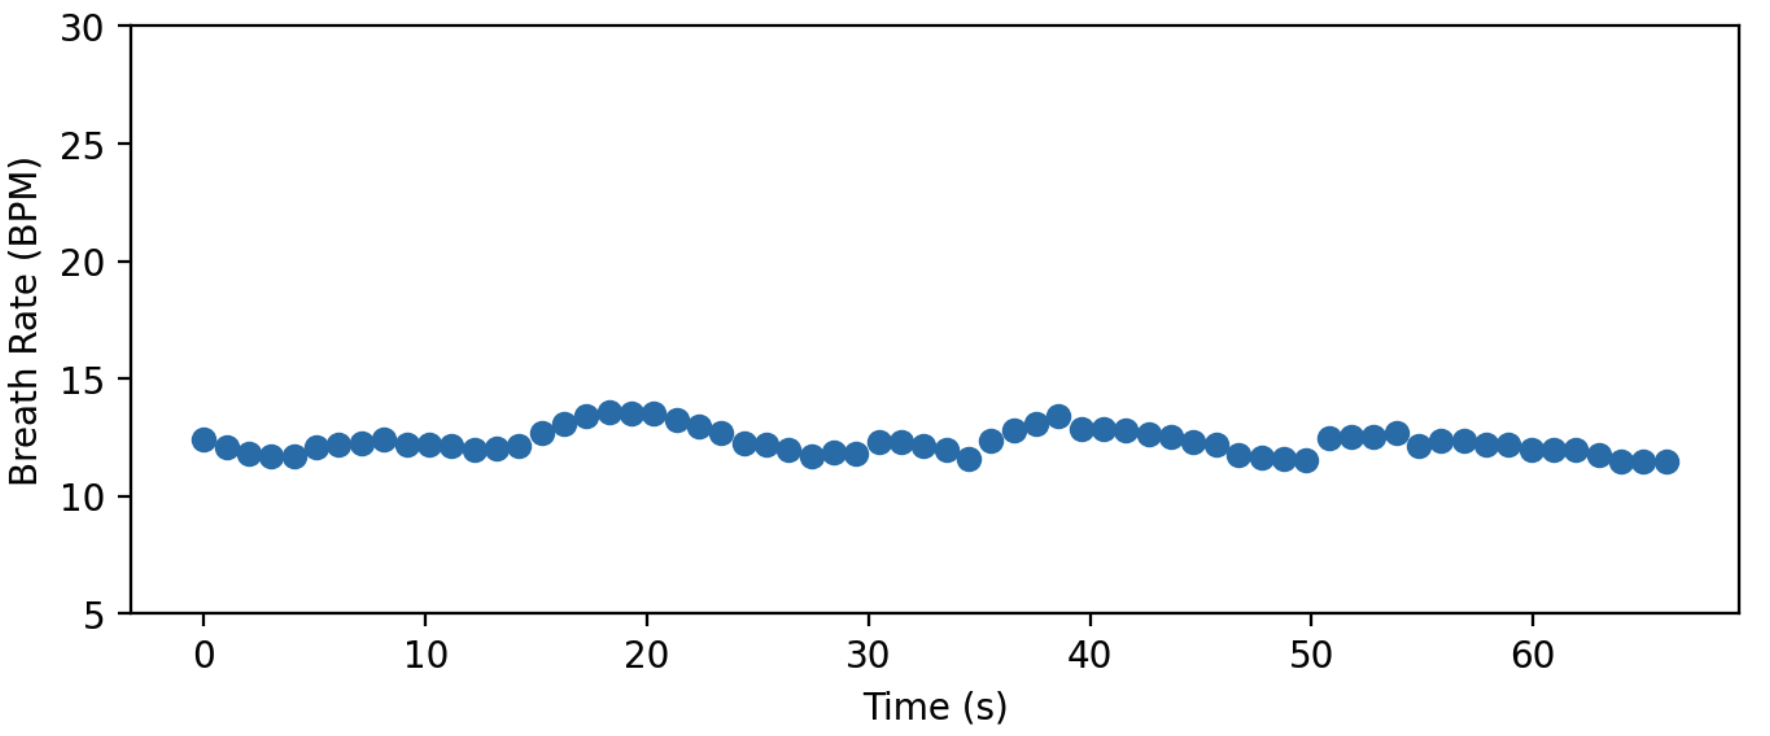
\includegraphics[width=0.5\linewidth]{fig/Exp.jpg}
    \caption{Estimated Respiration for \rm{193342.csv}.}
    \label{res1}
\end{figure}

\begin{figure}[!h]
    \centering
    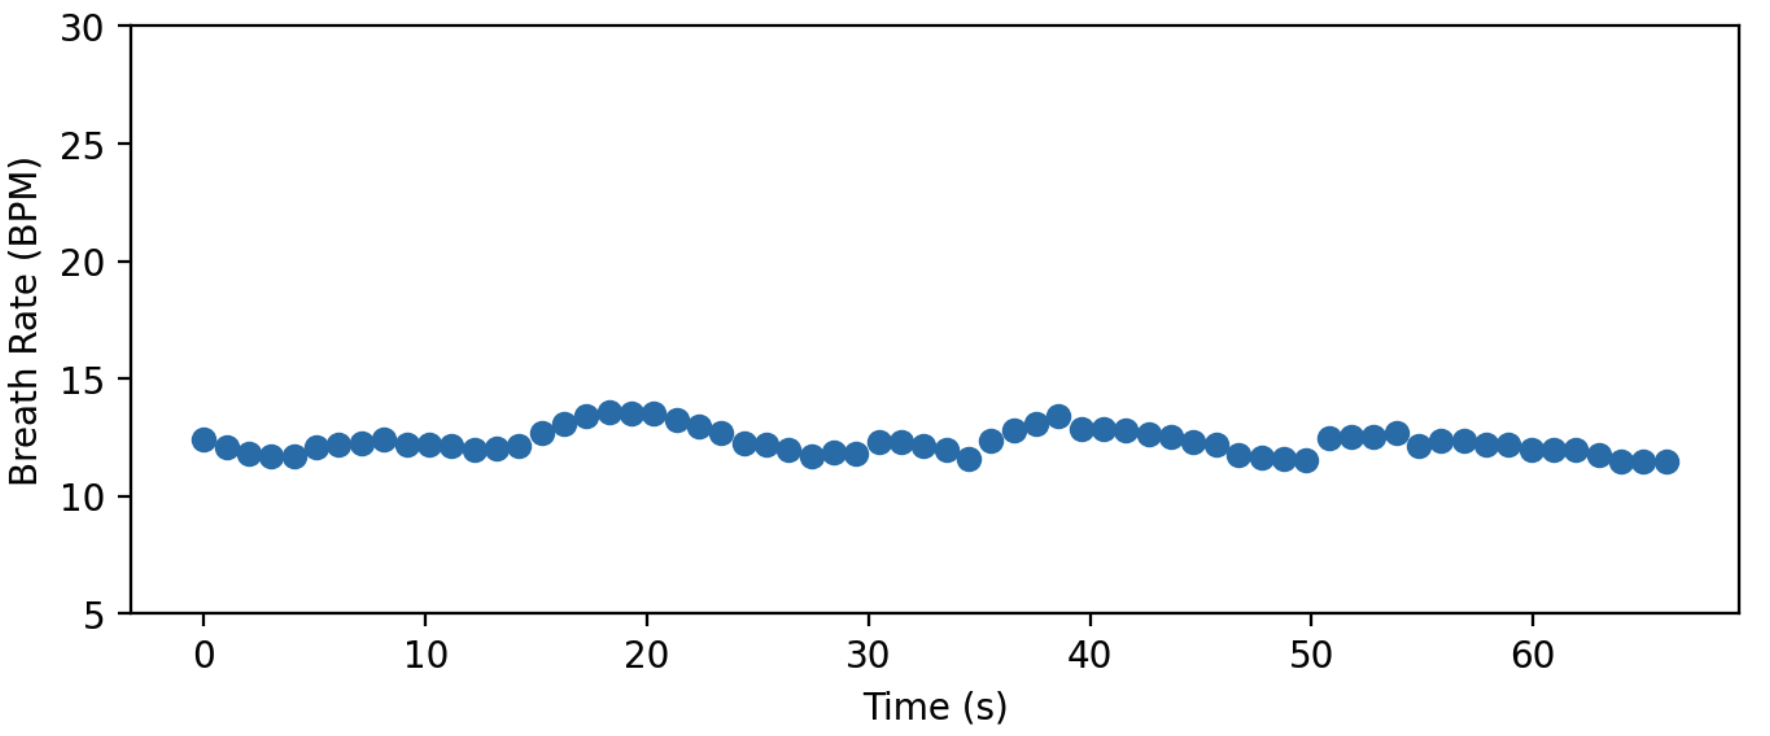
\includegraphics[width=0.5\linewidth]{fig/Exp.jpg}
    \caption{Estimated Respiration for \rm{200223.csv}.}
    \label{res2}
\end{figure}

\begin{figure}[!h]
    \centering
    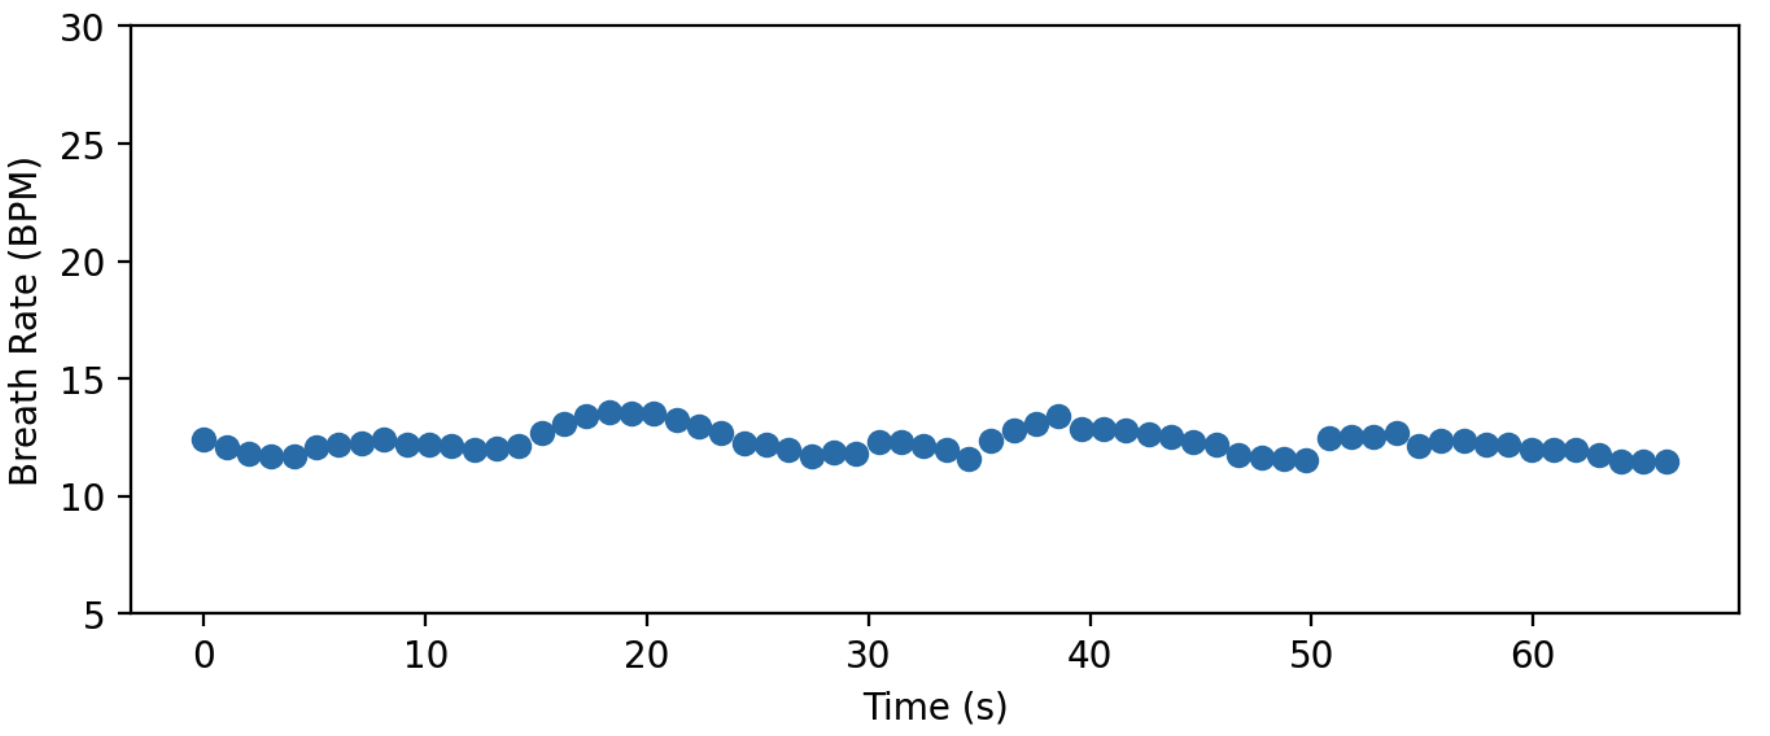
\includegraphics[width=0.5\linewidth]{fig/Exp.jpg}
    \caption{Estimated Respiration for \rm{201424.csv}.}
    \label{res3}
\end{figure}

\subsubsection{Motion Test}
Enter your result (1 for motion detected, 0 for no) in the table \ref{test motion}.

\begin{table}[!h]
\centering
\caption{Test Result of Motion Detection.}
\label{test motion}
    \begin{tabular}{cc|cc}
    \toprule
    \textbf{File Name} & \textbf{Result} & \textbf{File Name} & \textbf{Result} \\
    \midrule
    205713.csv &  & 205723.csv & \\
    205733.csv &  & 205803.csv & \\
    205822.csv &  & 205834.csv & \\
    205845.csv &  & 205855.csv & \\
    205906.csv &  & 205928.csv & \\
    205943.csv &  & 205958.csv & \\
    210036.csv &  & 210911.csv & \\
    210928.csv &  & 210942.csv & \\
    211010.csv &  & 211023.csv & \\
    211035.csv &  & 211055.csv & \\
    211107.csv & \\
    \bottomrule
    \end{tabular}
\end{table}


\clearpage
\newpage
\section{System Design}
\section{Results Visualization}
\section{Analysis}

% add whatever you want
